For any project to be successful it has to be well managed.
Deadlines must be set (and met), and the available time has to be rationed out to allow all parts of the project to be completed.

More research-based projects such as this one are slightly different, in that there is no formal set of requirements created before-hand.
Development on the code-base is very much an arbitrary process, with new ideas evolving and new avenues being explored at all times.
It is difficult to know at the outset which ideas will be successful, and if any new directions will emerge during the course of development.

Nevertheless, some deadlines were introduced in order to guide the project towards its end goal.
These deadlines were as follows:

\begin{enumerate}
	\item \textbf{Project brief submission} (Friday 19$^\text{th}$ October)
	\begin{itemize}
		\item Familiarization with basic computer vision algorithms
		\item Completion of test bed for shader implementations
	\end{itemize}
	
	\item \textbf{Interim report submission} (Friday 11$^\text{th}$ January)
	\begin{itemize}
		\item Completion of basic modelfitting framework (with one limb)
		\item Preliminary results generated
	\end{itemize}
	
	\item \textbf{Easter holiday} (Friday 14$^\text{th}$ March)
	\begin{itemize}
		\item Adaption of modelfitting framework for multiple limbs
		\item Graph plotting capabilities
	\end{itemize}
	
	\item \textbf{Final submission} (Thursday 8$^\text{th}$ May)
	\begin{itemize}
		\item Classification framework using DFTs
		\item Final results gathering
	\end{itemize}
\end{enumerate}

Overall I feel that these deadlines were kept to quite well.
Work on improving the algorithms continued until the very end of June - the final result of 90\% only being achieved a couple of weeks before the final deadline.
It would have been more useful to have obtained this result earlier, as then more time could have been invested in the report.

A gantt chart showing the actual work done on the project is given in Figure \ref{GanttChart}.
The data for this gantt chart was gathered from Subversion commit logs.
Graphs of Subversion commits per week and per hour are shown in Figure \ref{SVNGraphs}.

\begin{landscape}
	\begin{figure}[p]
		\centering
		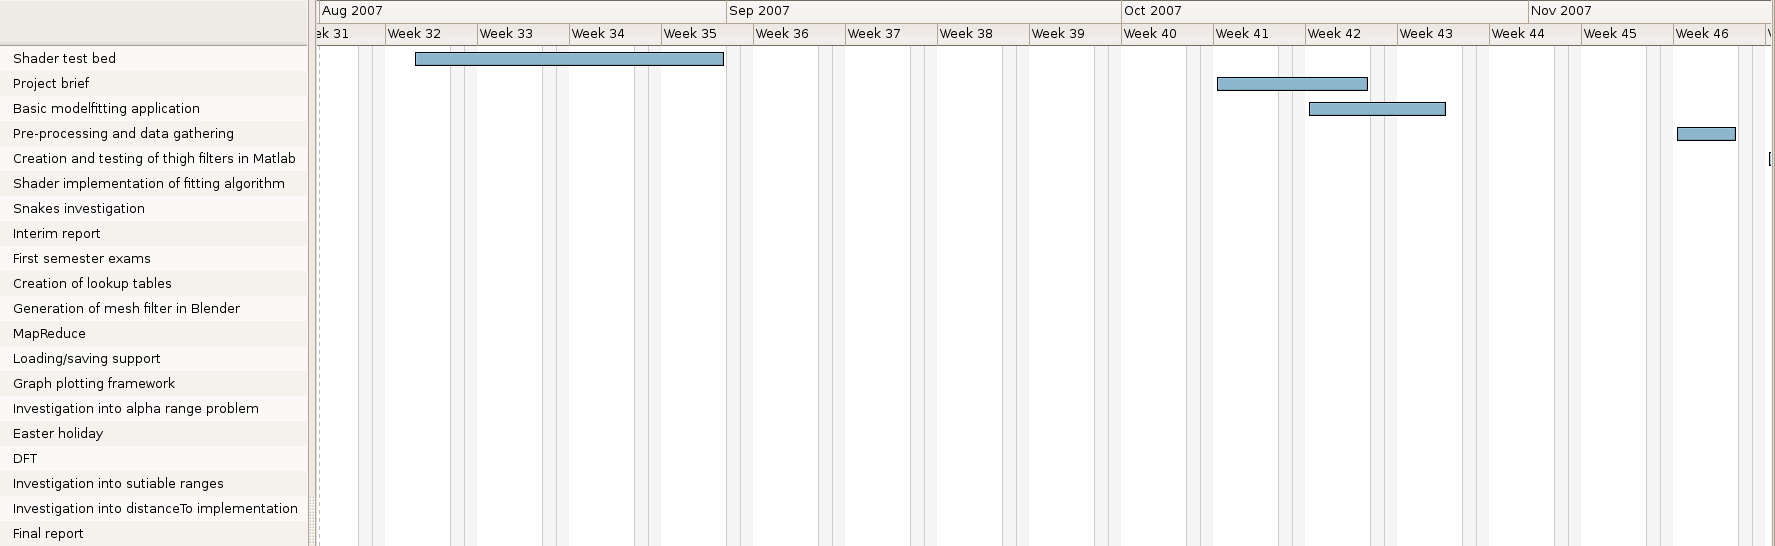
\includegraphics[width=21cm]{gantt.png}
	\end{figure}
	\begin{figure}[p]
		\centering
		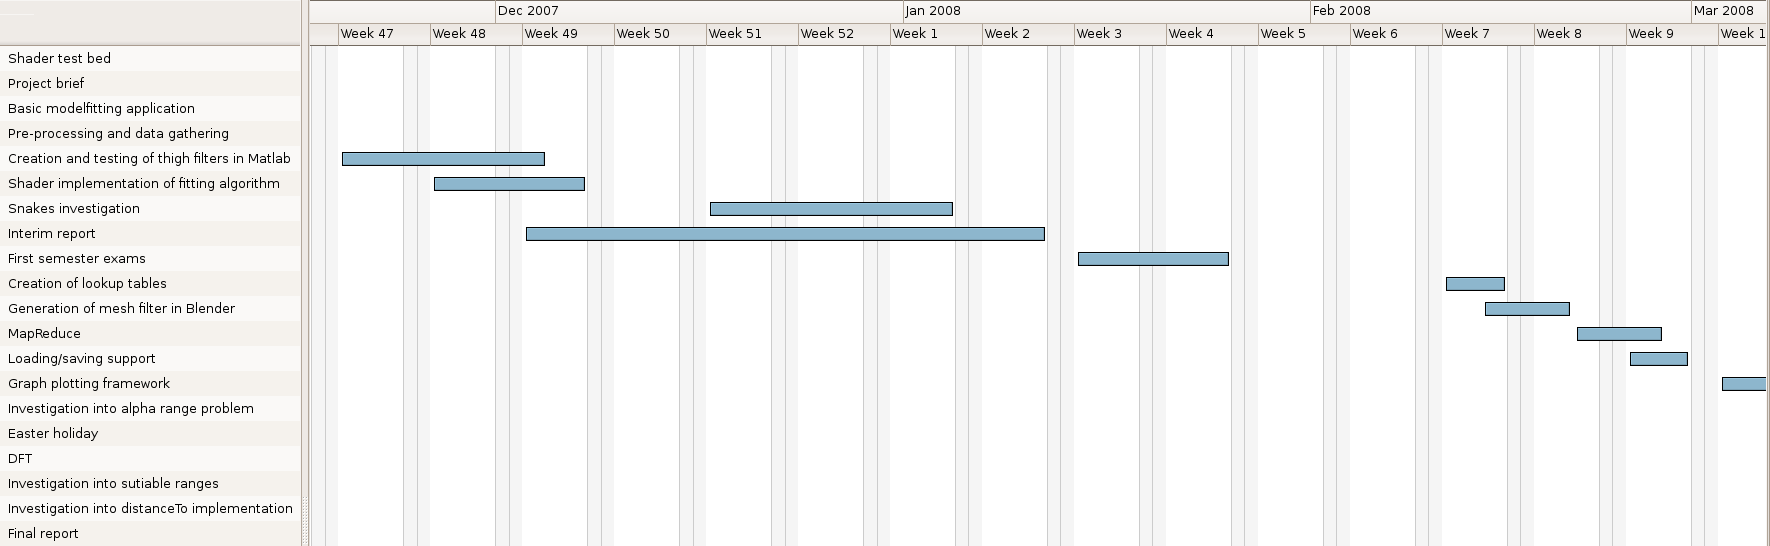
\includegraphics[width=21cm]{gantt2.png}
	\end{figure}
	\begin{figure}[p]
		\centering
		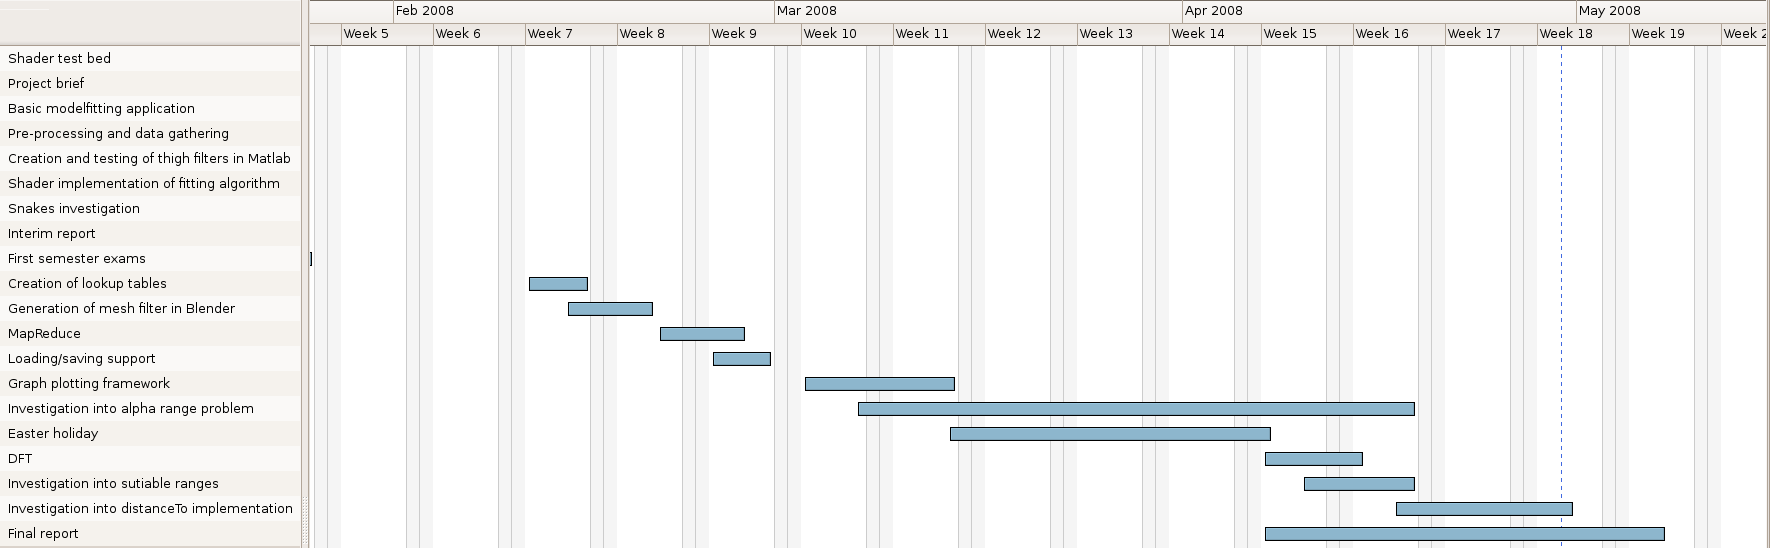
\includegraphics[width=21cm]{gantt3.png}
		\caption{Gantt chart.}
		\label{GanttChart}
	\end{figure}
\end{landscape}


\begin{figure}[p]
	\centering
	\subfloat[Per week]{\label{SVNPerWeek}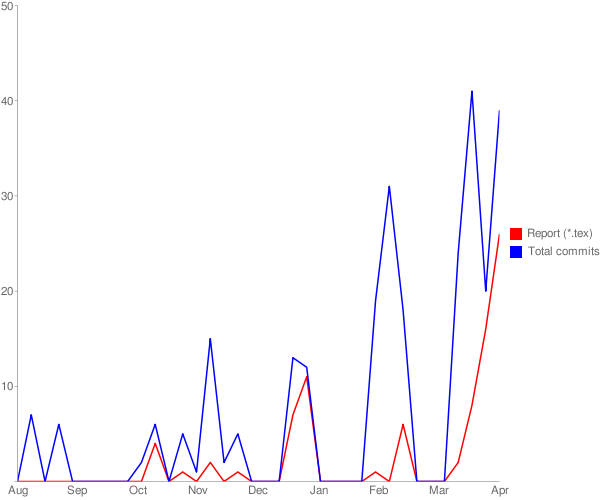
\includegraphics[width=10cm]{commits.png}}
	\qquad
	\subfloat[Per hour]{\label{SVNPerHour}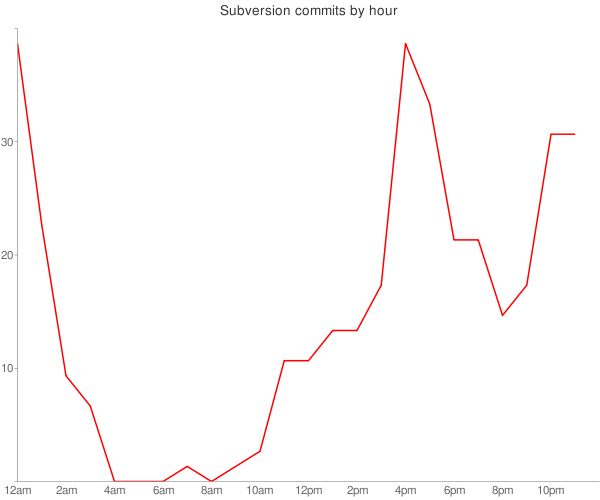
\includegraphics[width=10cm]{commitshour.png}}
	\caption{Subversion commits over time.
		This is representative of work done on the project.}
	\label{SVNGraphs}
\end{figure}
